\documentclass{article}
\usepackage{listings} \lstset{numbers=left, numbersep=5pt}
%\lstset{language=Perl} 

\oddsidemargin0mm
\evensidemargin0mm
\topmargin-20mm
\textwidth160mm
\textheight240mm
\parindent0pt

\newcommand{\C}{\mathbb{C}}
\newcommand{\N}{\mathbb{N}}
\newcommand{\Z}{\mathbb{Z}}
\newcommand{\Q}{\mathbb{Q}}
\newcommand{\R}{\mathbb{R}}
\newcommand{\K}{\mathbb{K}}
\usepackage[ngerman]{babel}   % provide non-american language - new german
\usepackage[ansinew]{inputenc} % nur fuer schoene Umlaute ;)
\usepackage{lscape}
\usepackage{multirow}
\usepackage{expdlist}
%\usepackage{bigstrut} % \bigstrut in Tabellenzeilen, deren hochgestellte Eintraege von der \hline drueber durchgestrichen werden
\usepackage{amsmath, amsthm, amssymb}
\usepackage{stmaryrd}
\usepackage{fancyhdr}
\usepackage{graphicx}
\newcommand{\serie}{4}

\pagestyle{fancy}
\fancyhf{}
\fancyhead[L]{Sebastian D\"orner (180766)} %Kopfzeile links
\fancyhead[C]{Algorithmische Geometrie} %zentrierte Kopfzeile
\fancyhead[R]{Mittwoch} %Kopfzeile rechts
\renewcommand{\headrulewidth}{0.0pt} %obere Trennlinie
\fancyfoot[C]{\thepage} %Seitennummer

\begin{document}
\begin{large}
\textbf{L"osung \"Ubung \serie}\\ \\
\end{large}
\textbf{Aufgabe 1}\\
Sei $GG(S)$ der Grabriel Graph von $S$ und $D(S)$ die Delauny-Triangulierung von $S$.\\
zz.: $\{p,q\}\in GG\Leftrightarrow \overline{pq} \in D(S) \wedge \overline{pq} \cap VR_S(p) \cap VR_S(q) \ne \emptyset$.\\
\begin{itemize}
\item[$\Rightarrow$] Sei $m=\frac{1}{2}(p+q)$ und $C=C(m,|\overline{pm}|)$. Dann ist $C$ der Kreis mit Durchmesser $\overline{pq}$ und enth\"alt nach Voraussetzung keinen anderen Punkt aus $S$ in seinem Inneren. D.h. es gibt einen Punkt $m$, sodass $C = C_S(m)$ nur $p$ und $q$ enth\"alt, aber keinen anderen Punkt aus $S$. Nach einem Satz aus der Vorlesung (V3-30) ist dann aber $\overline{pq}\in D(S)$.\\
Es bleibt zu zeigen, dass $\overline{pq} \cap VR_S(p) \cap VR_S(q) \ne \emptyset$. Da $p\in VR_S(p)$ und $q \in VR_S(q)$ beginnt die Strecke $\overline{pq}$ in $VR_S(p)$ und endet in $VR_S(q)$. Angenommen sie schneidet die Voronoikante $VR_S(p) \cap VR_S(q)$ nicht, dann muss es einen indirekten \"Ubergang von $VR_S(p)$ nach $VR_S(q)$ \"uber mindestens eine weitere Voronoizelle geben, dies sei $VR_S(r)$. $VR_S(r) \cap \overline{pq}$ enth\"alt mindestens die zwei \"Uberg\"ange zu benachbarten Voronoizellen, d.h. $|VR_S(r)\cap\overline{pq}|\geq 2$. Da $VR_S(r)$ und $\overline{pq}$ konvex sind, folgt $rel\,int(VR_S(r)\cap \overline{pq}) \ne \emptyset$. Sei also $x\in rel\,int(VR_S(r)\cap \overline{pq})$, d.h. $VR_S(r)$ ist die einzige Voronoizelle, in der $x$ enthalten ist. Sei o.B.d.A. $d(x,p) = \min\{d(x,p), d(x,q)\}$. Mit $d(x,r) < d(x,p)$ folgt aber $r \in C(x, d(x,r))\subset C(x,d(x,p)) \subseteq C(m,d(m,p)) = C$, im Widerspruch zur Voraussetzung, dass $C$ keinen Ort au\ss er $p$ und $q$ enth\"alt. Somit war unsere Annahme falsch und $\overline{pq} \cap VR_S(p) \cap VR_S(q) \ne \emptyset$
\item[$\Leftarrow$] Sei $m \in \overline{pq} \cap VR_S(p) \cap VR_S(q)$, dann ist $d(m,p)=d(m,q)$ (auf der gemeinsamen Voronoikante). Sei weiterhin $C=C(m, d(m,p))$. Es ist zu zeigen, dass $C$ keinen weiteren Ort aus $S$ in seinem Inneren enth\"alt. Angenommen es gibt einen weiteren Ort $x\in int\,C$. Dann ist $d(m,x)<d(m,p)$, d.h. $m\not\in VR_S(p)$ im Widerspruch zur Voraussetzung. Also war die Annahme der Existenz von $x$ falsch und $\{p,q\} \in GG(S)$.\qed
\end{itemize}
\textbf{Aufgabe 2}\\
\begin{figure}[h]
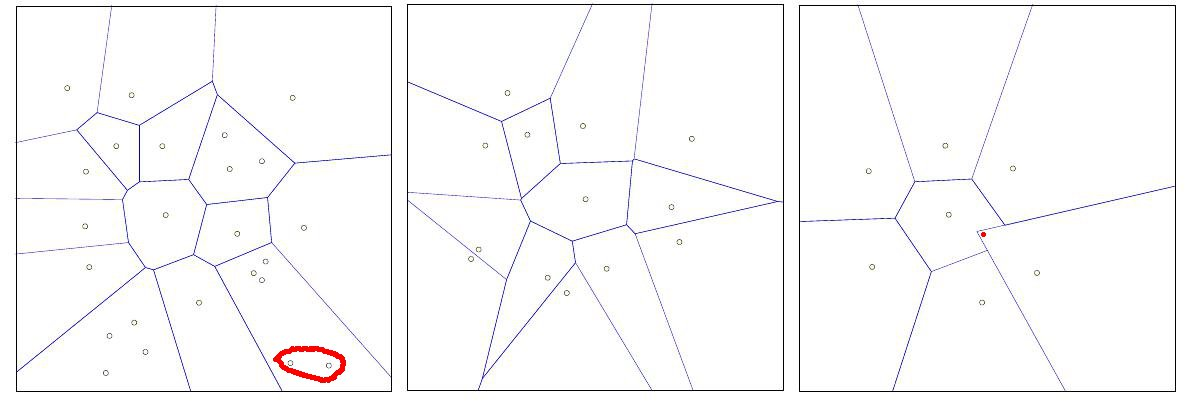
\includegraphics[width=\textwidth]{a2}
\end{figure}\\
In der linken Abbildung befinden sich mehrere Orte in der selben Voronoiregion. Dies kann nicht sein, da sich jeder Ort in seiner eigenen Voronoiregion befindet ($d(x,x)=0$), es ist also kein g\"ultiges Voronoidiagramm. \\Bei der mittleren Abbildung scheint es sich um ein g\"ultiges Voronoidiagramm zu handeln. Ohne aber die genauen Koordinaten aller eingezeichneten Objekte zu kennen, k"onnen wir das nicht zweifelsfrei nachweisen.\\In der rechten Abbildung ist der rot eingezeichnete Punkt n\"aher am mittleren Ort als an dem Ort, in dessen Voronoiregion er liegt. Somit ist es ebenfalls kein g\"ultiges Voronoidiagramm.\\
\textbf{Aufgabe 3}
\begin{itemize}
\item[(a)] Zun\"achst zeigen wir, dass es kein Gebiet gibt, das von Kanten aus $T$ umschlossen ist. Angenommen es g\"abe ein solches Gebiet $G$, dann w\"urde es mindestens eine Voronoiregion $VR_S(q)$ komplett beinhalten, also $VR_S(q) \subseteq G$. Da eine Voronoiregion der Schnitt von Halbr\"aumen bez\"uglich Bisektoren ist und beim Hinzuf\"ugen eines neuen Punktes $p_i$ f\"ur jeden bereits vorhandenen Punkt nur ein Bisektor dazukommt, ist der Teil, der von den alten Voronoiregionen wegf\"allt, genau die neue Voronoiregion $VR_{S\cup\{p_i\}}(p_i)$. Damit folgt $VR_S(q) \subseteq G \subseteq VR_{S\cup\{p_i\}}(p_i)$. Wir betrachten den Bisektor von $q$ und $p_i$ und seine Lage bez\"uglich $VR_S(q)$.
\begin{itemize}
\item[Fall 1:] Der Bisektor schneidet oder ber\"uhrt $VR_S(q)$. Dann gibt es auf der $q$ zugewandten Seite des Bisektors noch Punkte in $G$. Diese liegen nach Def. des Bisektors aber n\"aher an $q$ als an $p_i$ und sind somit nicht Teil von $VR_{S\cup\{p_i\}}(p_i)$. Dies steht aber im Widerspruch zu $G \subseteq VR_{S\cup\{p_i\}}(p_i)$.
\item[Fall 2:] Der Bisektor schneidet oder ber\"uhrt $VR_S(q)$ nicht. Dann liegt $VR_S(q)$ vollst\"andig auf der $q$ zugewandten Seite des Bisektors. Dann ist $VR_S(q) \cap VR_{S\cup\{p_i\}}(p_i) = \emptyset$, im Gegensatz zu $VR_S(q) \subseteq VR_{S\cup\{p_i\}}(p_i)$.
\end{itemize}
Da beide F\"alle auf Widerspr\"uche f\"uhren, muss die Annahme der Existenz einer solchen Region $G$ falsch gewesen sein. Somit ist T kreisfrei.
Wir zeigen nun, dass $T$ ein Baum ist. Alle Punkte von $T$ haben zu mindestens zwei Orten in $S$ den minimalen Abstand, da sie Teil des Voronoi-Skeletts sind. Die Schnittpunkte von $T$ mit $VR_{S\cup\{p_i\}}(p_i)$ haben den gleichen minimalen Abstand au\ss erdem zu $p_i$. Somit liegen diese Schnittpunkte genau an den Ecken der neuen Voronoiregion. $T$ unterteilt $VR_{S\cup\{p_i\}}(p_i)$ in Subgebiete. Wenn $T$ nicht zusammenh\"angend w\"are, dann g\"abe es zwei Kanten von $bd\,VR_{S\cup\{p_i\}}(p_i)$, die an das gleiche Subgebiet grenzen. Im Ursprungs-Diagramm (vor Hinzuf\"ugen von $p_i$) waren die zu den Kanten geh\"orenden Voronoizellen dann aber verbunden. Dies kann aber nicht sein, weil zu den zwei Kanten aus $bd\,VR_{S\cup\{p_i\}}(p_i)$ auch zwei Orte geh\"oren m\"ussen. Also muss die Annahme, $T$ sei nicht zusammenh\"angend, falsch gewesen sein.\\
Also ist $T$ kreisfrei und zusammenh\"angend, d.h. $T$ hat eine baumartige Struktur.
\item[(b)] Seien $p_a$, $p_b$ und $p_c$ die Orte mit minimalem Abstand zu $v$ mit $d(v,p_a) = d(v,p_b) = d(v,p_c)$.
\begin{eqnarray*}
&& \text{v wird entfernt}\\
&\Leftrightarrow& VR_{S\cup\{p_i\}}(p_i)\text{ ist die einzige Voronoizelle von $S\cup\{p_i\}$, die }v\text{ enth\"alt}\\
&\Leftrightarrow & d(v,p_i) < d(v,p_a)\\
&\Leftrightarrow & p_i \in int\,C(v,d(v,p_a)) = int\,C(v)
\end{eqnarray*}\qed
\end{itemize}
\end{document}
